\documentclass[8pt]{extarticle}
\title{}
\author{Avinash Iyer}
\date{}

%font setup
%
%\usepackage[math]{anttor}

%paper setup
\usepackage{geometry}
\geometry{letterpaper, portrait, margin=1in}
\usepackage{fancyhdr}

%symbols
\usepackage{amsmath}
\usepackage{amssymb}
\usepackage{hyperref}
\usepackage{gensymb}

\usepackage[T1]{fontenc}
\usepackage[utf8]{inputenc}

%chemistry stuff
\usepackage[version=4]{mhchem}
\usepackage{chemfig}

%plotting
\usepackage{pgfplots}
\usepackage{tikz}

%\usepackage{natbib}

%graphics stuff
\usepackage{graphicx}
\graphicspath{ {./images/} }

%a useful command
\newcommand{\plain}[1]{\textrm{#1}}

%code stuff
%when using minted, make sure to add the -shell-escape flag
%you can use lstlisting if you don't want to use minted
%\usepackage{minted}
%\usemintedstyle{pastie}
%\newminted[javacode]{java}{frame=lines,framesep=2mm,linenos=true,fontsize=\footnotesize,tabsize=3,autogobble,}
%\newminted[cppcode]{cpp}{frame=lines,framesep=2mm,linenos=true,fontsize=\footnotesize,tabsize=3,autogobble,}

\usepackage{listings}
\usepackage{color}
\definecolor{dkgreen}{rgb}{0,0.6,0}
\definecolor{gray}{rgb}{0.5,0.5,0.5}
\definecolor{mauve}{rgb}{0.58,0,0.82}

\lstset{frame=tb,
	language=Java,
	aboveskip=3mm,
	belowskip=3mm,
	showstringspaces=false,
	columns=flexible,
	basicstyle={\small\ttfamily},
	numbers=none,
	numberstyle=\tiny\color{gray},
	keywordstyle=\color{blue},
	commentstyle=\color{dkgreen},
	stringstyle=\color{mauve},
	breaklines=true,
	breakatwhitespace=true,
	tabsize=3
}
\pagestyle{fancy}
\fancyhf{}
\rhead{Avinash Iyer, Tobias Searcy-Jorgensen}
\lhead{Lab 2}
\begin{document}{
\section*{Experiment I}
\begin{quote}
	The goals of this experiment are to learn how to use a motion sensor and to test whether you understand graphs.
	
	A motion sensor sends out ultrasonic pulses and times their reflection off a nearby object.  The computer software detects the position of the object and can then plot graphs of Position vs. Time and Velocity vs. Time for the object.  Plug the motion sensor into the USB port of the computer, then open PASCO Capstone with the icon on the computer’s desktop. 
\end{quote}
\subsection*{Question 1}
\begin{quote}
	Determine the range of the motion sensor.
	
	Stand near the sensor and move back slowly in a straight line.  Note the range for which there is a signal on the Position vs. Time graph. Your motion must be within this range in order for the sensor to detect your motion.  Remember that any other object (table, other people, etc.) that lies inside the sensor’s “sound cone” may lead to false readings, so be sure that there is nothing between the sensor and the object being tracked. 
	
	\textit{\underline{If the motion sensor fails to perform satisfactorily, try one or more of the following suggestions:}}
	\begin{itemize}
		\item \textit{Ensure that the target object is not closer than 15 cm.}
		\item \textit{Remove interfering objects near the target object or the motion sensor.}
		\item \textit{Switch the range switch to the other setting.}
		\item \textit{Adjust the aim left, right, up, or down.  In some cases, the motion sensor works better when it is aimed slightly to the side or above the target in order to exclude interfering objects.}
		\item \textit{Improve the target by adding a larger or harder surface to reflect the ultrasonic waves.}
		\item \textit{Increase or decrease the sample rate.}
	\end{itemize}
	Include the Position vs. Time graph and report your result for the range in the space below.
\end{quote}
\begin{center}
	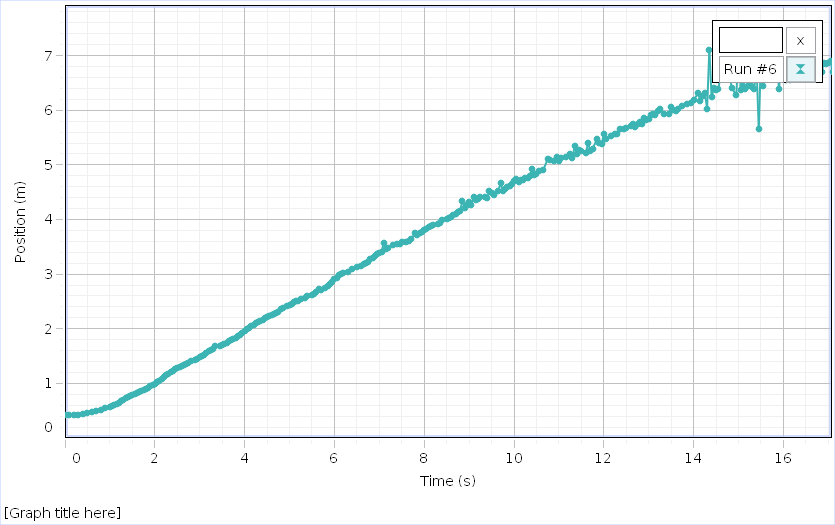
\includegraphics[width=10cm]{Lab2Image1_1}
\end{center}
The maximum range on the acoustic motion sensor is approximately 6.25 meters.
\subsection*{Question 2}
\begin{quote}
	Next, try moving in different ways while recording your motion with Position vs. Time and Velocity vs. Time graphs simultaneously.  Perform the following experiments: \\
	(a) Stand still, then walk forward at a steady pace, then stand still again. \\
	(b) Walk forward at a steady pace for 4 seconds, and then walk backward for 2 seconds at a steady but faster pace. \\
	(c) Walk forward at a steady pace for 2 seconds, and then continually increase your speed. \\
	
	Include the three sets of graphs in the space below (Copy the selected set of graphs choosing “Copy Display” from the “Display” option, and then paste it in your Word document, or simply print the graphs using “File” – “Print”. Do not save the graphs as PASCO Capstone files (“.cap”) using “File” - “Save Experiment As”, because you will need the PASCO Capstone program to open them).
\end{quote}
\pagebreak 
\begin{center}
	Experiment A: \\
	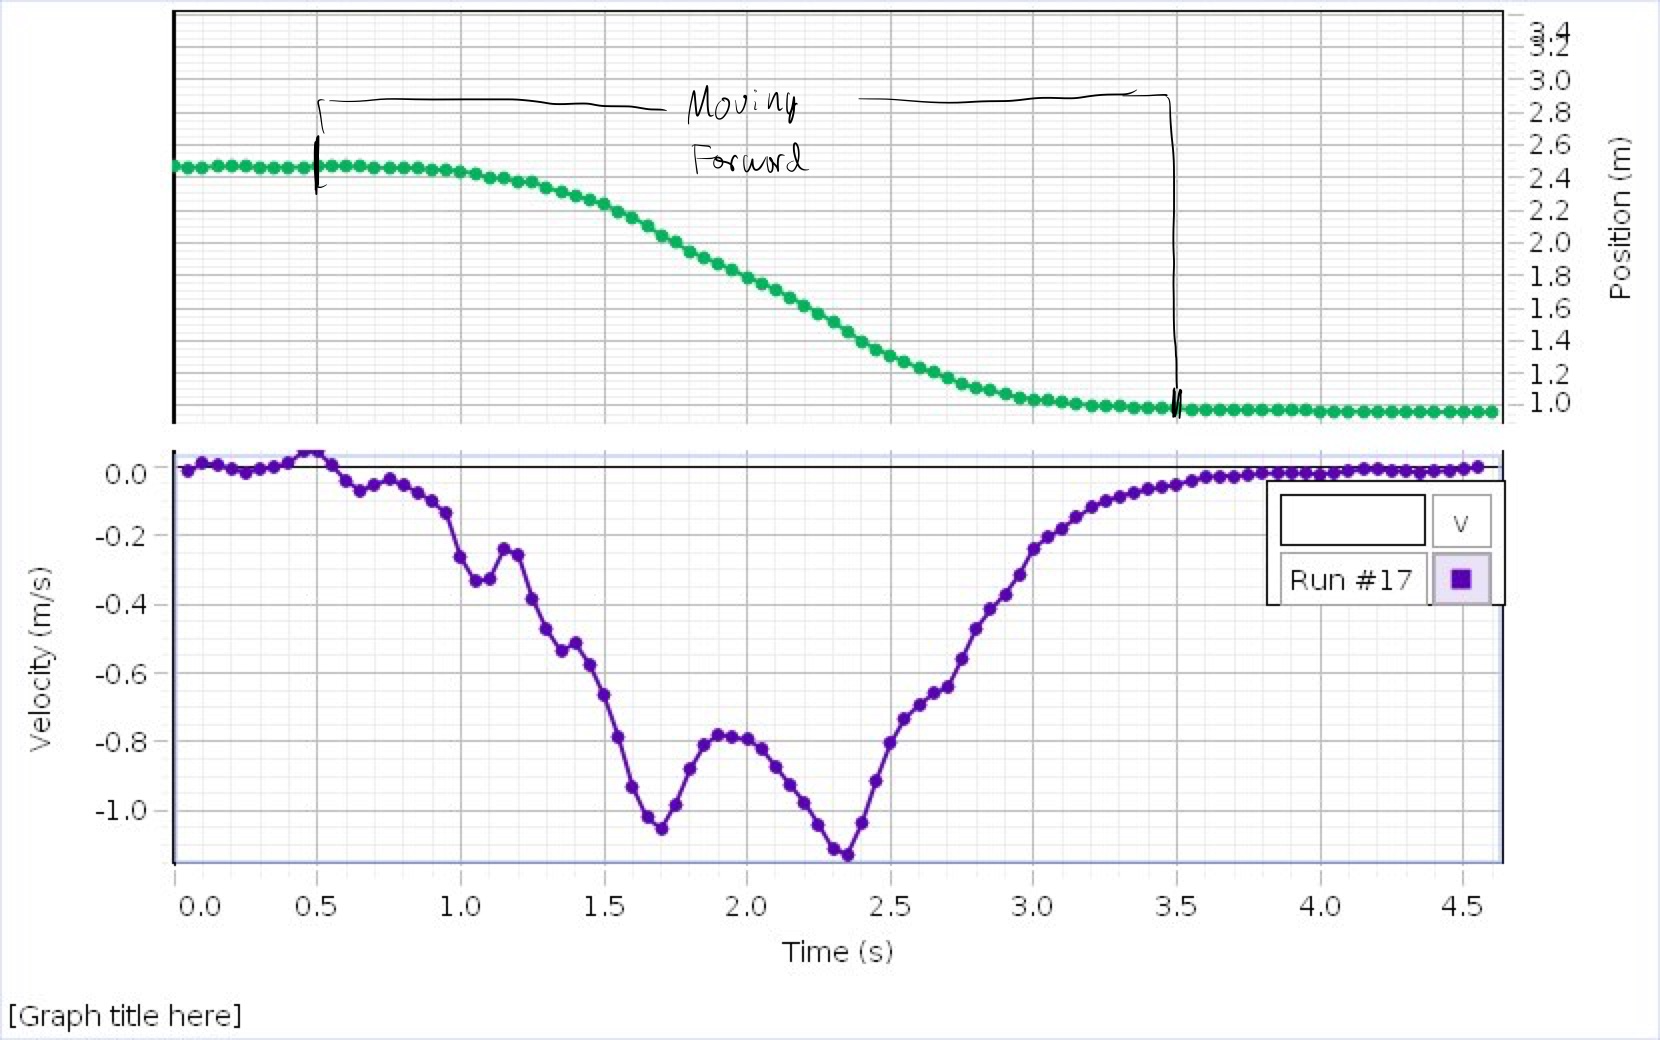
\includegraphics[width=10cm]{Lab2Image1_2_1}\\
	Experiment B:\\
	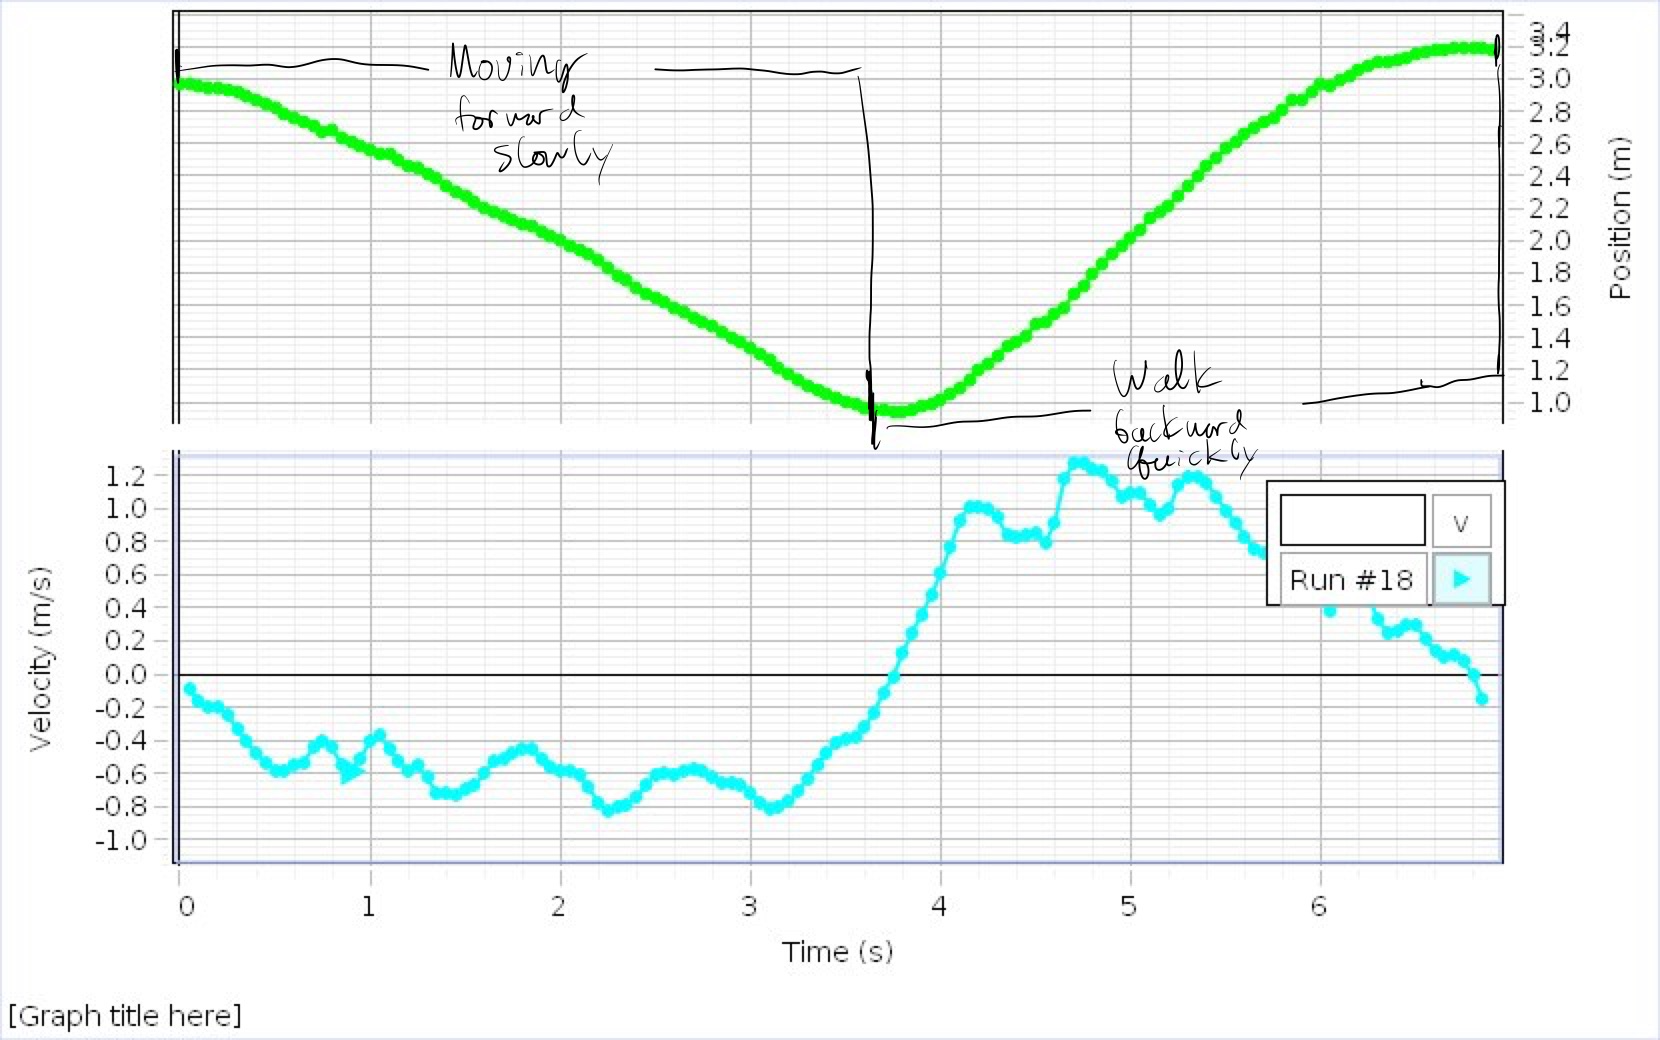
\includegraphics[width=10cm]{Lab2Image1_2_2}\\
	Experiment C: \\
	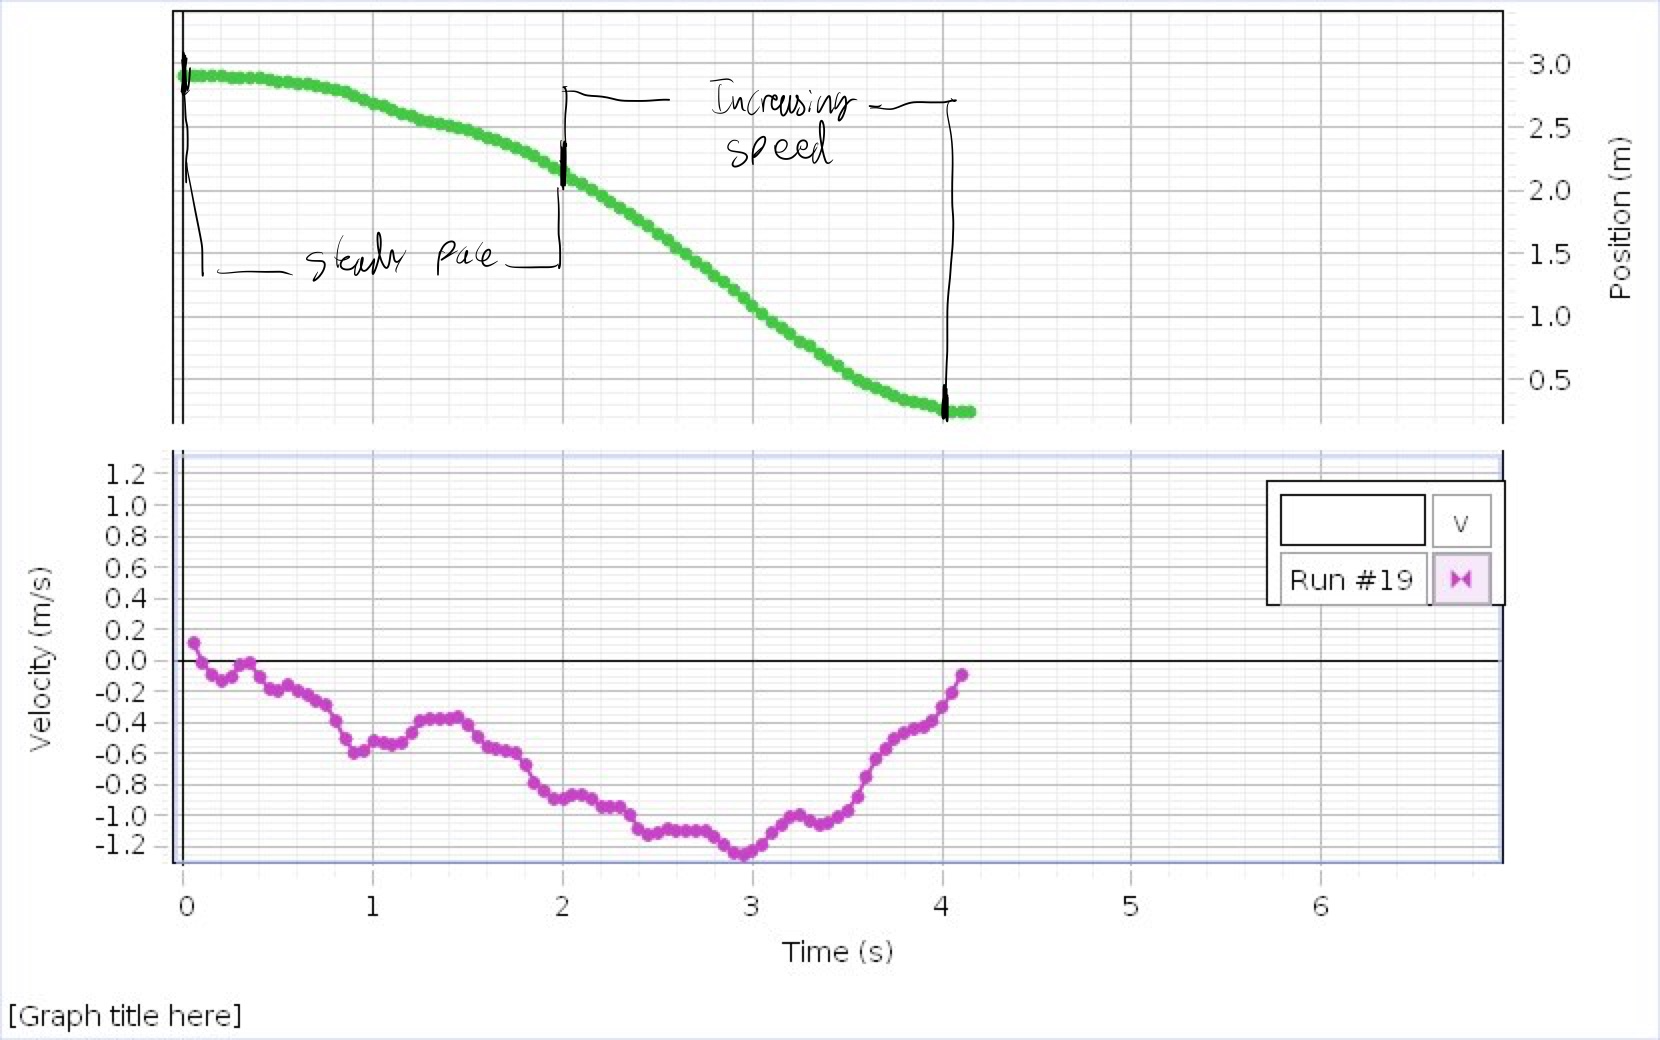
\includegraphics[width=10cm]{Lab2Image1_2_3}
\end{center}
In all three cases, the slopes on the position vs. time graph is approximately equal to the values on the velocity vs. time graph.
\subsection*{Question 3}
Your next task is to move in such a way that the graphs produced by your motion match a set of fixed, pre-determined graphs.  Open File Explorer (yellow folder in the taskbar)), then go to Windows (C:)\textbackslash Program Files (x86)\textbackslash Pasco Scientific\textbackslash DataStudio\textbackslash EZScreens\textbackslash EZMotion.exe. \\
(a) After the display launches, find the selection buttons for the four different Match Graph courses, along with the Match Mode On/Off button.  Click on the first graph (top left) to turn on Match Mode and display the graph.  If the display says that no sensor is attached, unplug the USB cable from the computer tower, and then plug it back in. \\
(b) When you click the Start button, you will have a 5-second countdown to position yourself in front of the motion sensor.  The computer will count down the 5 seconds, and then it will automatically begin data collection.  Data collection will end automatically after 10 seconds. \\
(c) Before you perform the experiment, you need to decide how you should move in order to produce graphs that match those that are on the screen.  After you are sure about how you want to move, perform the experiment.  If the graph produced by your motion does not match the provided graph, discuss possible reasons.  Revise and repeat the experiment. \\
(d) The Match Score is a representation of how closely your movements matched the course given by the computer.  Try to get it as high as possible. \\
(e) For each of the four Match Graph courses, print the final graph that is closest to the given one. \\
(f) On one of the four graphs, explain why your graphs never have “corners” like the ones that you are trying to match.
Include all four graphs in the space below: \\
\begin{center}
	Experiment 1: \\
	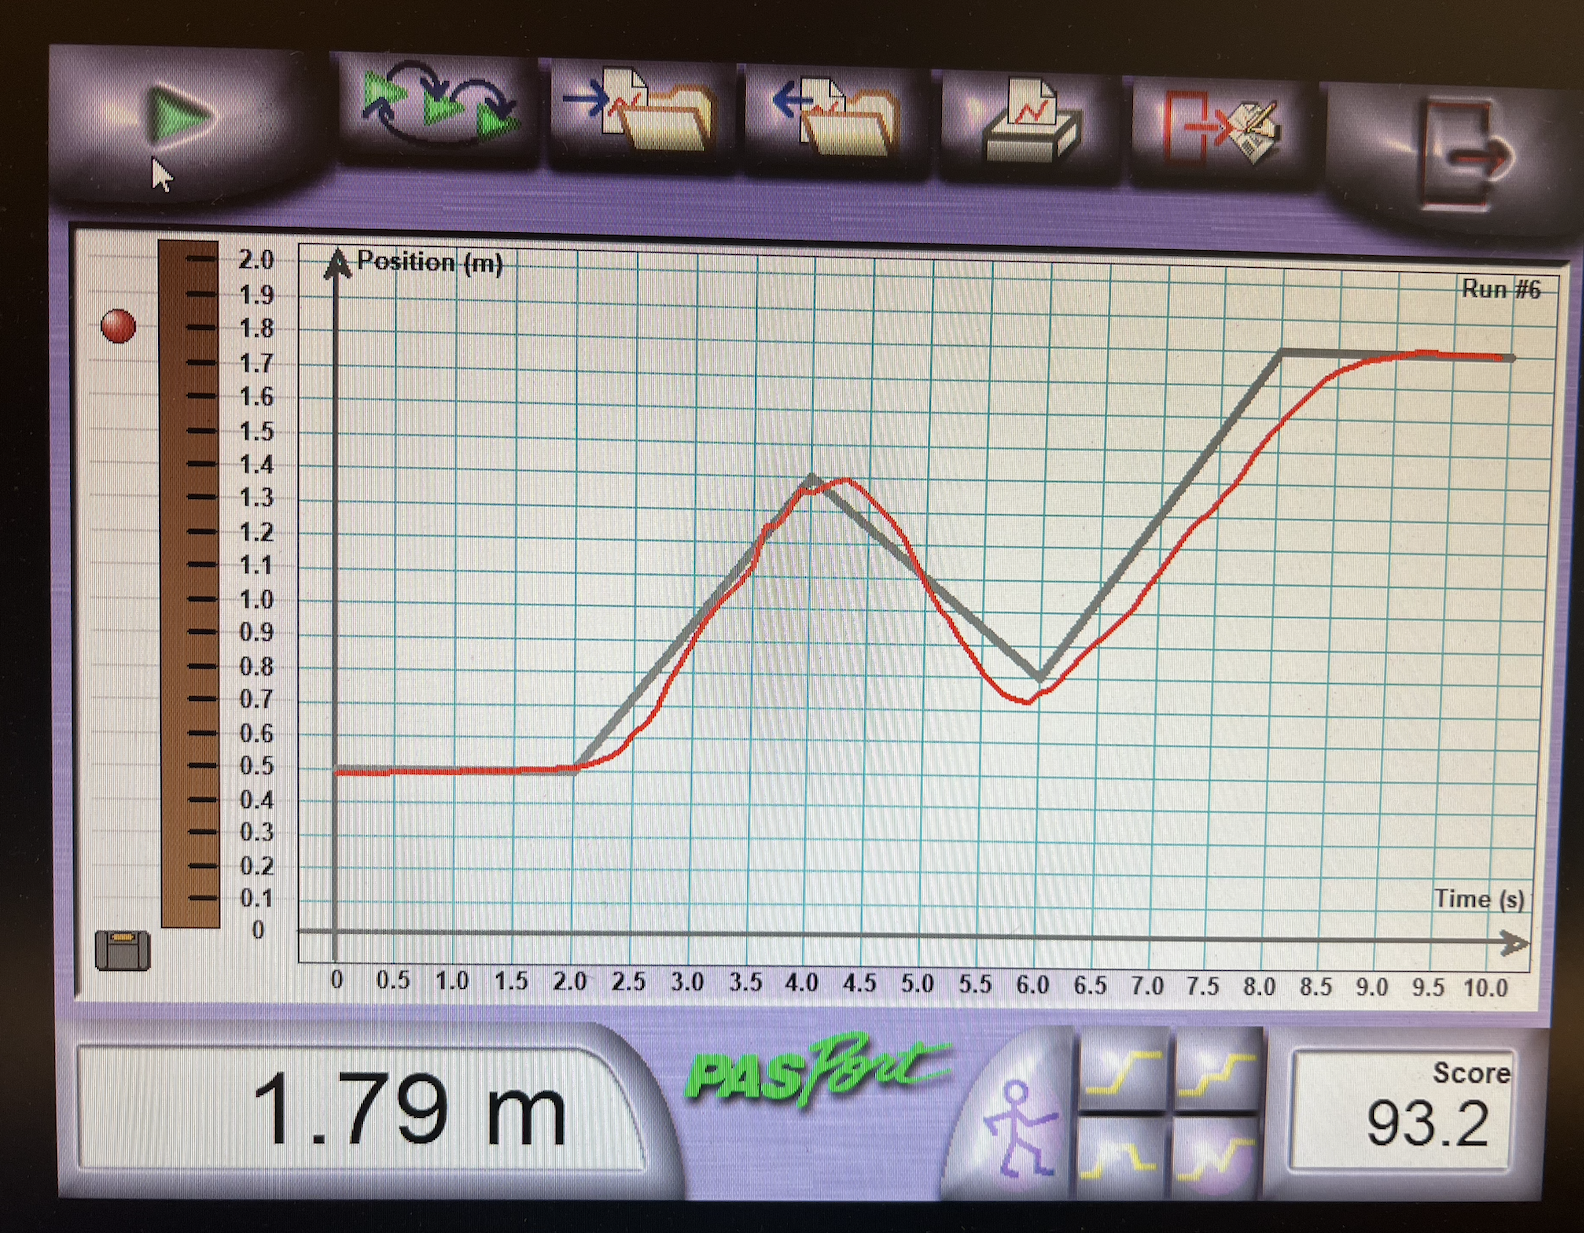
\includegraphics[width=10cm]{Lab2Image1_3_1}\\
	Experiment 2:\\
	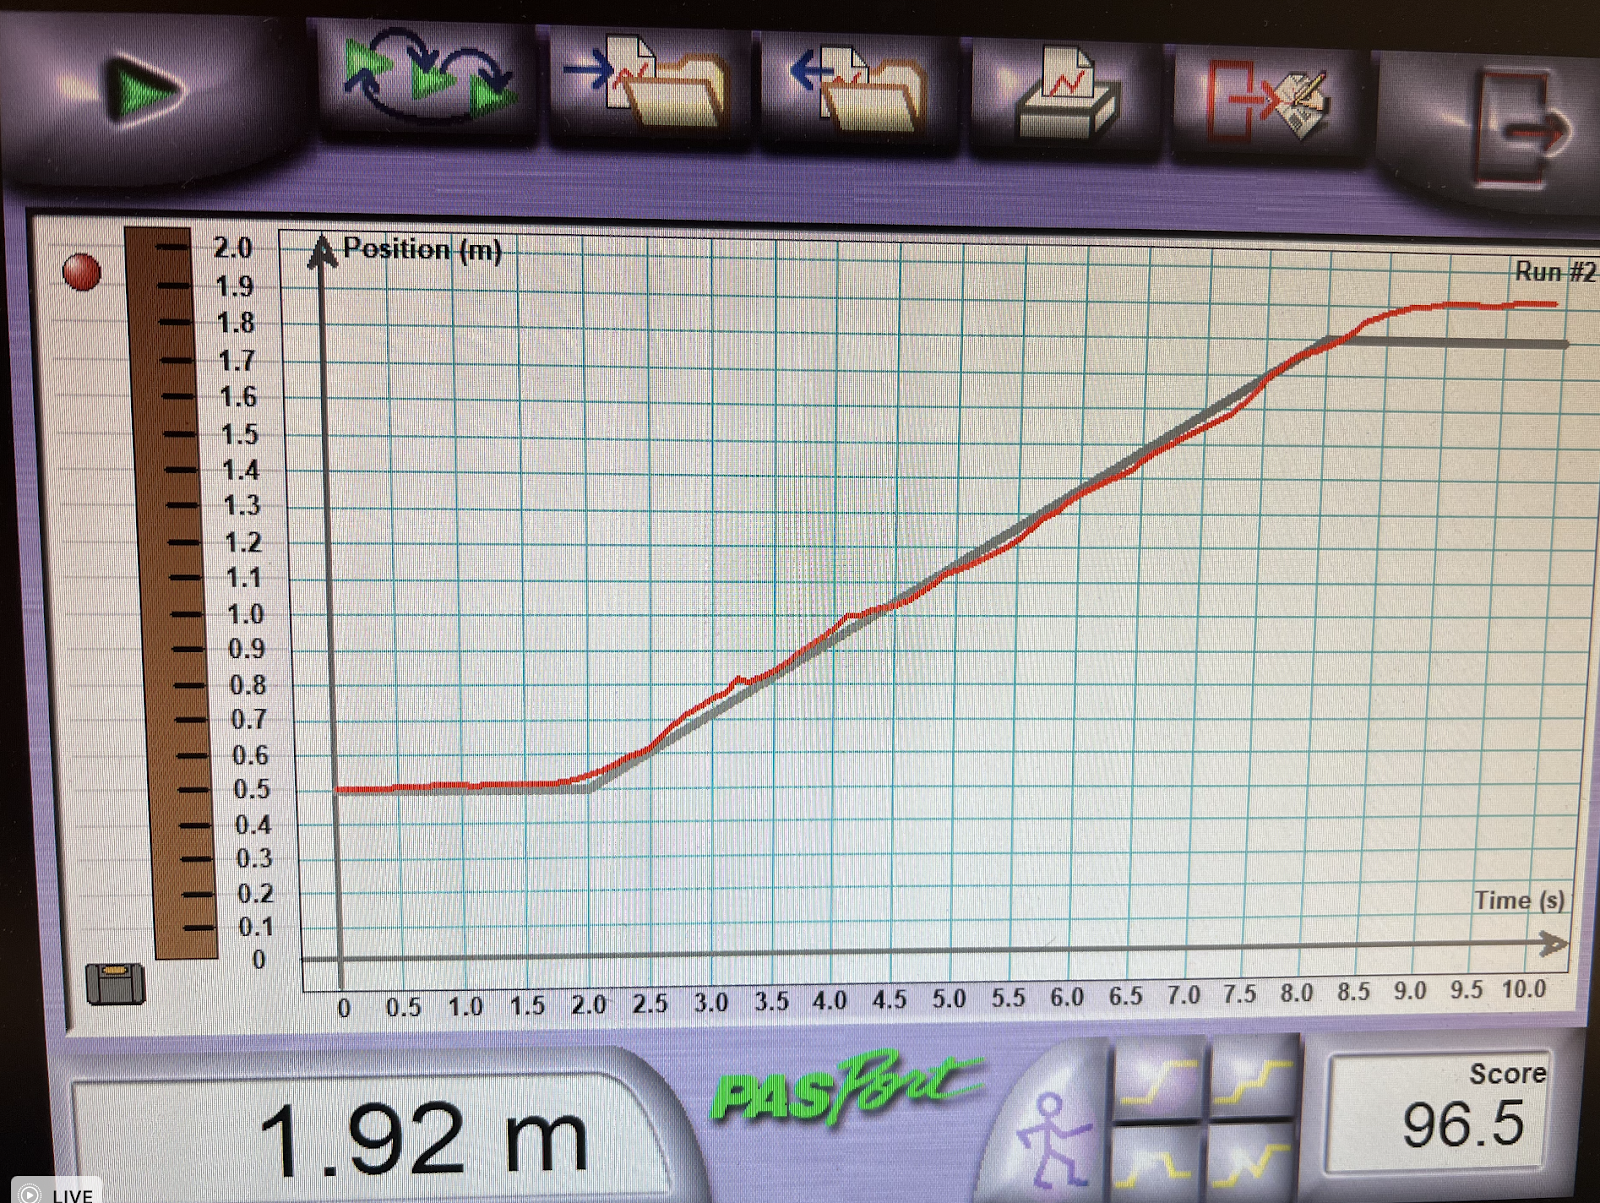
\includegraphics[width=10cm]{Lab2Image1_3_2}\\
	\pagebreak
	Experiment 3:\\
	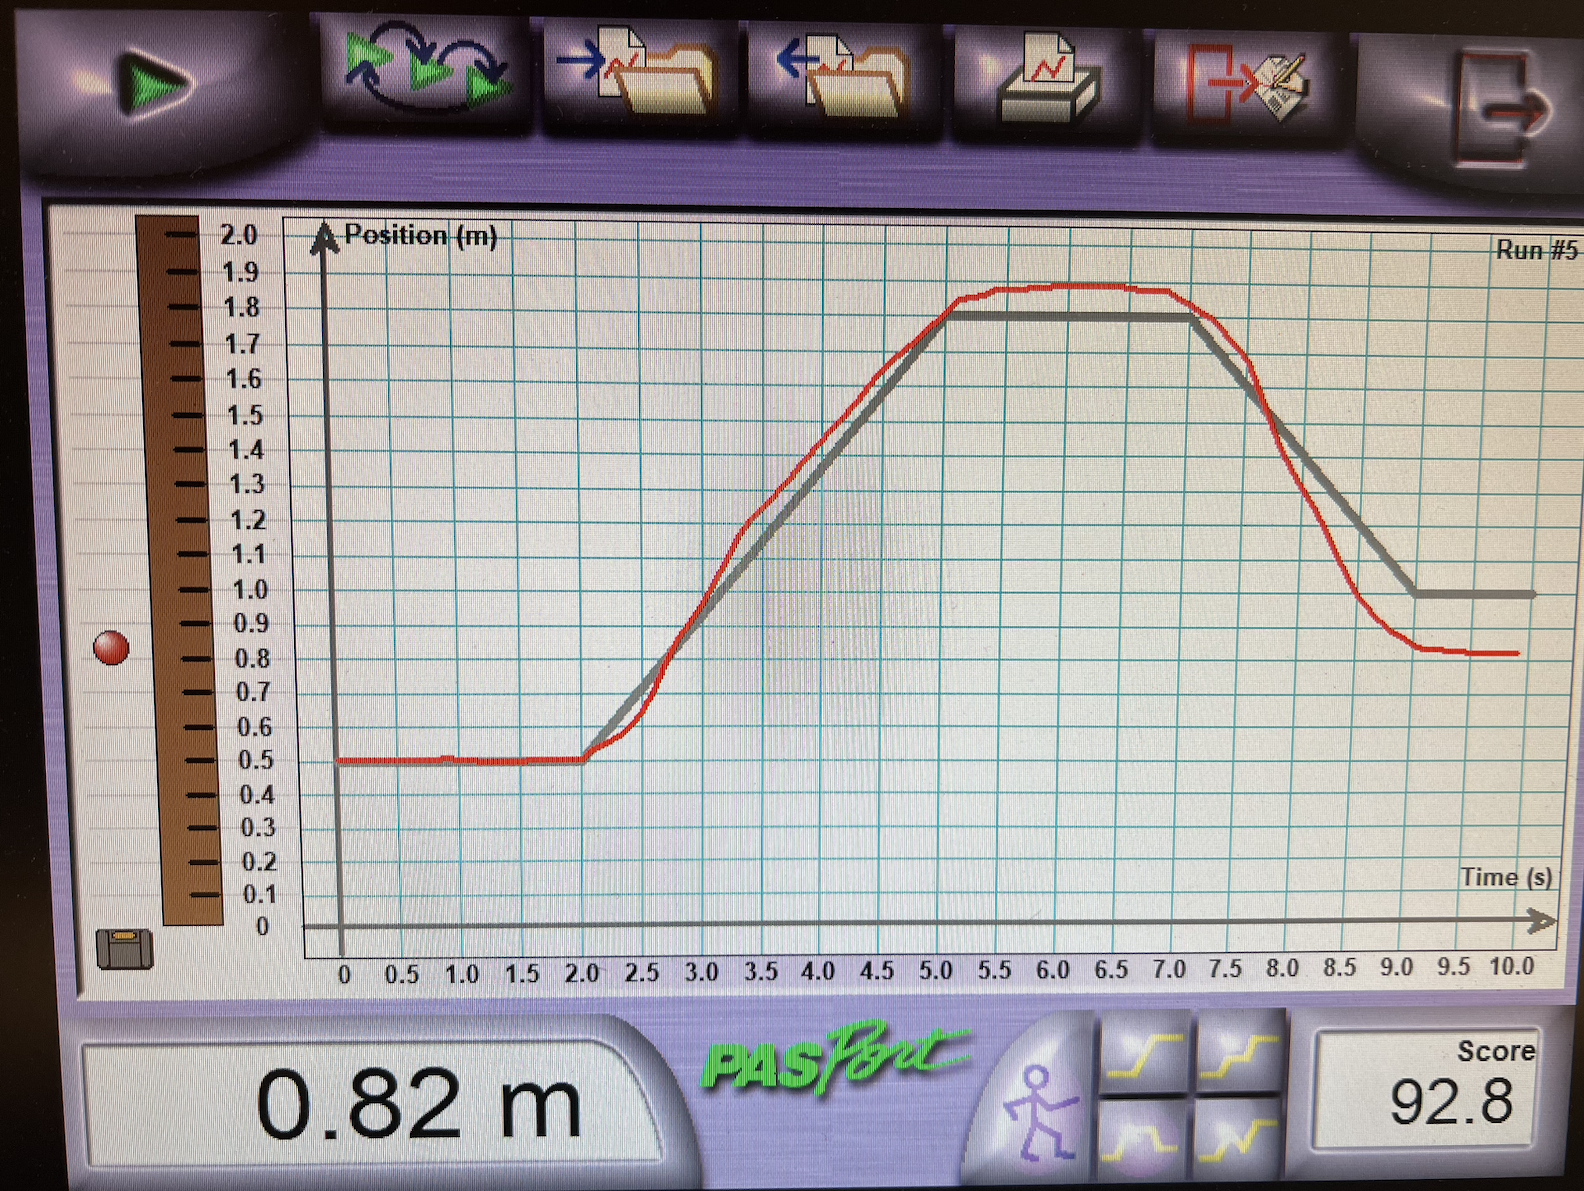
\includegraphics[width=10cm]{Lab2Image1_3_3}\\
	Experiment 4:\\
	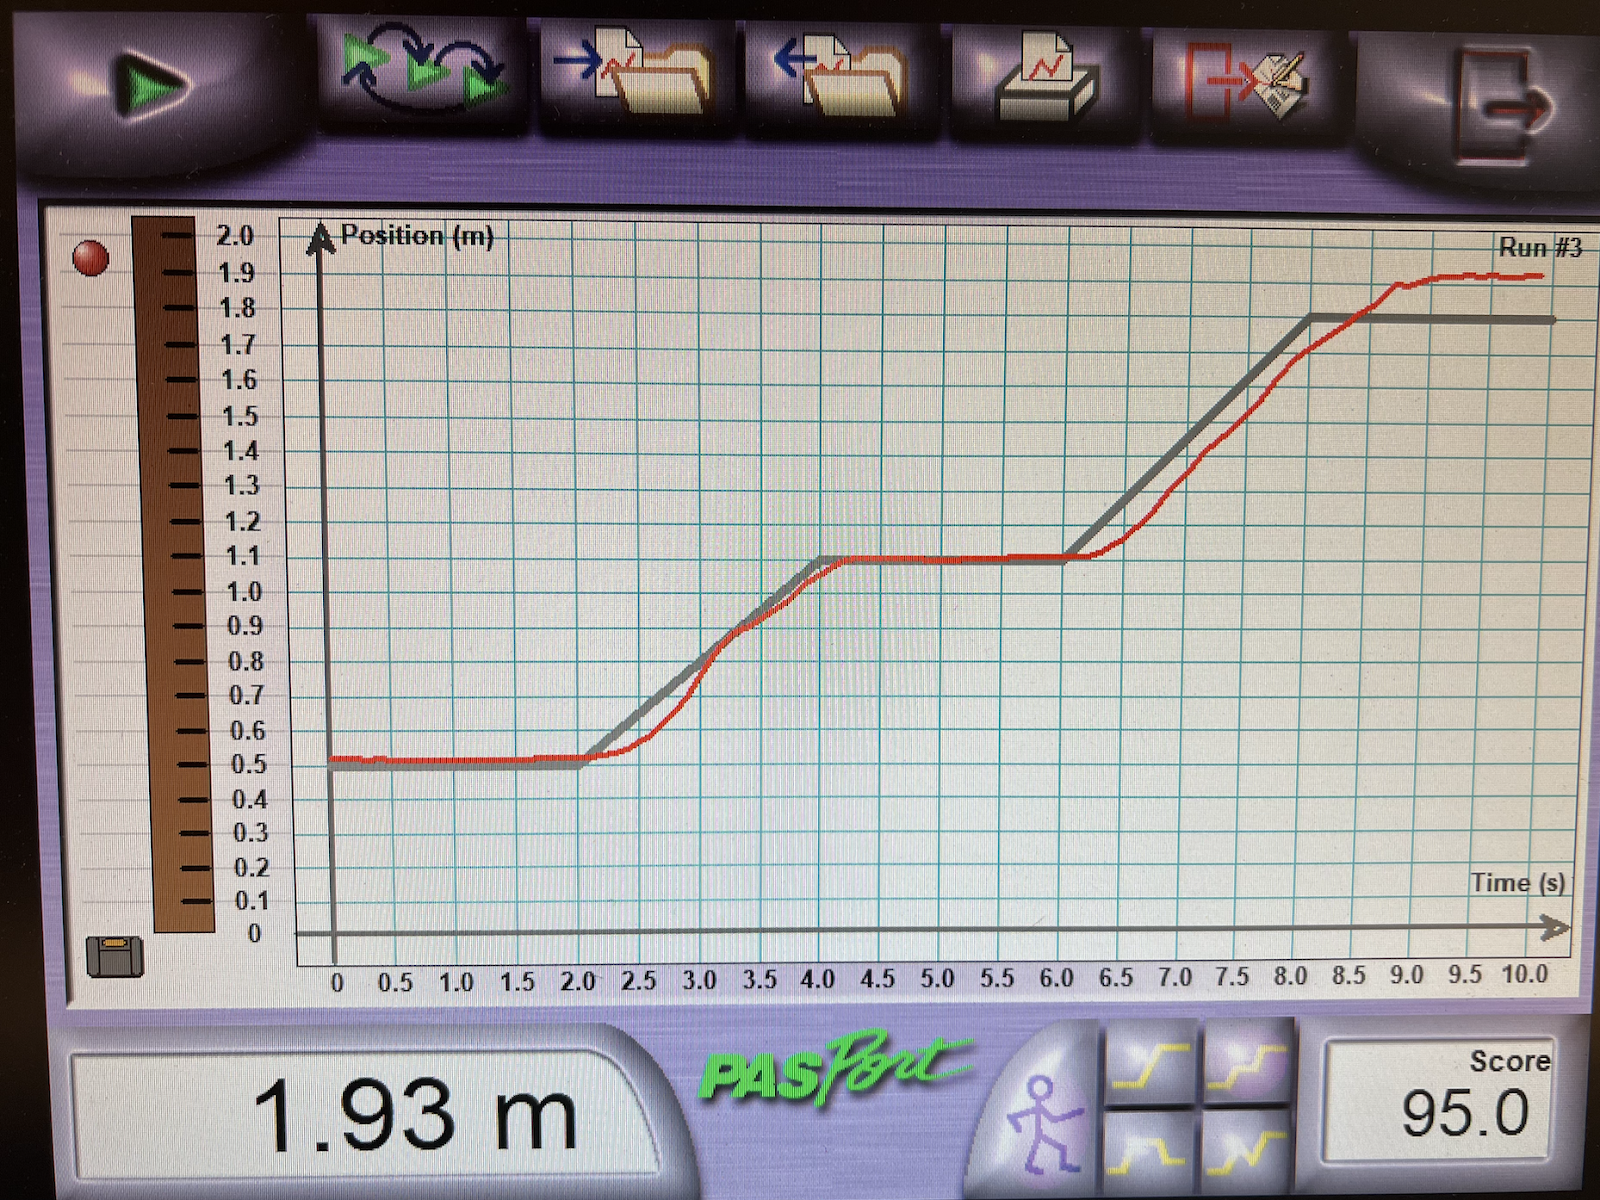
\includegraphics[width=10cm]{Lab2Image1_3_4}
\end{center}
For experiment 3, the primary reason the graph of motion does not have corners is that it is essentially impossible for one to change from zero velocity to constant forward or backward velocity immediately.
\section*{Experiment II: Comparison of Methods for Quantitative Description of a Cart's Motion}
\begin{quote}
	The goals of this experiment are to measure the speed of an object using three different methods and to compare the different measurement techniques: using a motion sensor, a photogate, and a stopwatch.
	
	\textbf{CAUTION:  Do not place the cart on the air track unless the air is turned on.  Use with care to not scratch or nick the surface of the air track.  Any protrusions on the surface will impede the motion of the cart.}
	
	First, make sure that the air track is level.  In a perfect world, this would mean that a cart placed anywhere on the track would remain at rest when released (with the air turned on).  In the real world, the air track is not perfectly level and the cart will move.  Release the cart from rest in the middle of the air track.  If the cart moves very slowly, then the track is level enough to proceed.  If the cart moves quickly or shows a noticeable acceleration, ask your instructor to show you how to level the track.
	
	Use a rubber band stopper at one end of the air track as a launcher to propel the cart.  Pull it back as far as possible, and then release the cart.  \textbf{Be sure that the rubber band is stretched the same amount every time!}
	
	The goal of the experiment is to determine the speed of the cart immediately after it is launched.  Keep this in mind as you arrange your apparatus, make your measurements, and analyze your data.
\end{quote}
\subsection*{Part 1: Motion Sensor Method}
\begin{quote}
	\textit{\textbf{Note:} When using the motion sensor, make sure that it is not getting reflections from some unwanted object.  To exclude interference with the reflecting surface of the track, the sensor should be aimed slightly above the cart and parallel to the air track.  The cart’s sail should be aligned \textbf{perpendicular} to the direction of motion in order to increase the target area for the ultrasonic pulses.}
	
	Use the motion sensor and the PASCO Capstone software to simultaneously produce graphs of Position vs. Time and Velocity vs. Time for the launched cart.
\end{quote}
\subsubsection*{Subpart 1}
\begin{quote}
	Present and describe the Position vs. Time and Velocity vs. Time graphs.
\end{quote}
\begin{center}
	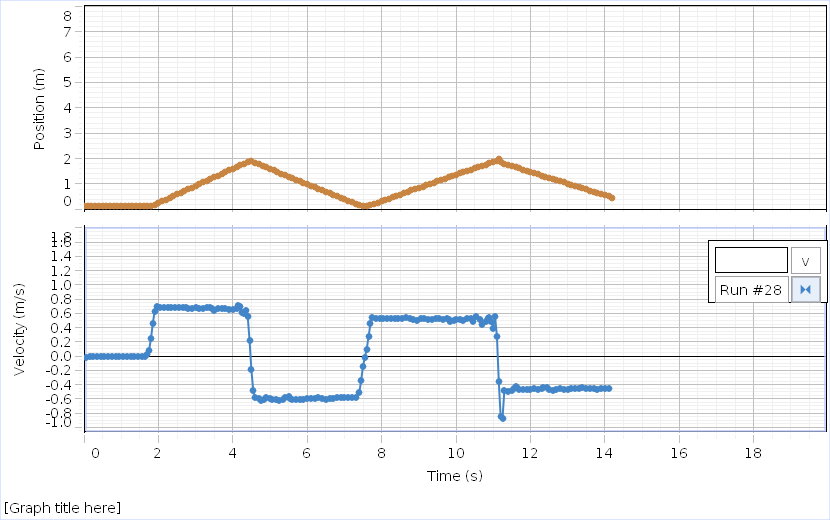
\includegraphics[width=10cm]{Lab2Image2_1_1}
\end{center}
The position graph describes a cart that is moving forwards and backwards with the same speed but with different directions. These are shown in the velocity vs. time graph with the opposite sign but same magnitude of velocity.
\subsubsection*{Subpart 2}
\begin{quote}
	Highlight the portion of the Velocity vs. Time graph where the cart was moving with a constant speed. Use PASCO Capstone’s Statistics tools to calculate the average value of the data, and its uncertainty, for the highlighted region of the graph.  The Mean will tell you the average speed in the highlighted region, and the Standard Deviation can be used as the uncertainty in the average speed in this case.  Present the graph (with the Mean and Standard Deviation shown) below. 
\end{quote}
\begin{center}
	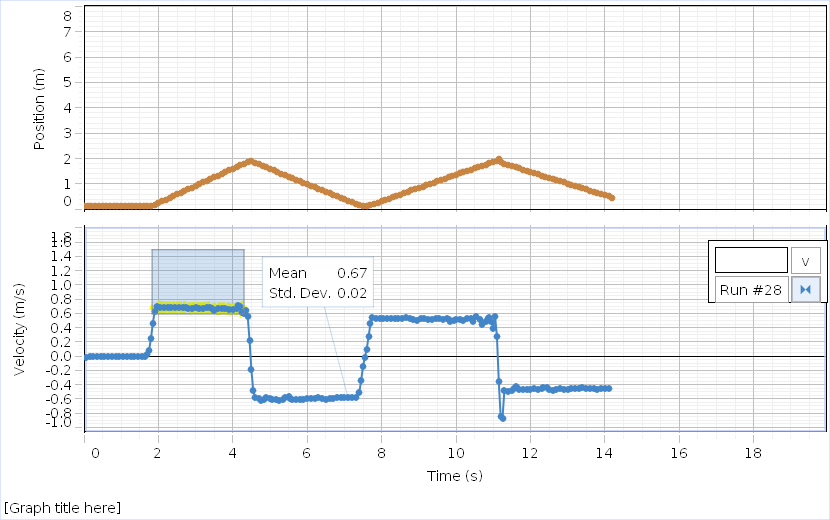
\includegraphics[width=10cm]{Lab2Image2_1_2}
\end{center}
\subsubsection*{Subpart 3}
\begin{quote}
	Report the final result of your measurement in an appropriate format.  The final result and its uncertainty should have the correct units and the correct number of decimal places and significant figures.
\end{quote}
\[ v = 0.67\pm 0.02~\plain{m/s} \]
\subsubsection*{Subpart 4}
\begin{quote}
	Describe another method that could be used to determine the speed of the cart from the Position vs. Time graph. (You do not have to do it, just describe how it could be done).
\end{quote}
We could also calculate the slope of one of the sections of the graph via linear regression or some other method, and from that determine a velocity.
\subsection*{Part 2: Photogate Method}
\begin{quote}
	The photogate is a timing device that is useful for measuring events that happen faster than you can time by hand. It is also useful for determining the speed of an object. The photogate consists of an infrared diode and a photocell. Timing occurs while the infrared beam between the diode and the photocell is interrupted. You can’t see the beam, but it is there. The numbers on the display show the time of the event in seconds.
	To determine speed with the photogate:
	\begin{itemize}
		\item Set the timer to GATE mode. Set the photogate to the “1 ms” setting. Use the RESET button to zero the photogate reading. The photogate’s reading will always be in seconds. Measure the length of the object (the cart’s sail) that is breaking the beam. This object must have definite edges, and the photogate must be positioned so that the object passes through the beam at a right angle to the beam.
		\item Since speed equals distance divided by time, divide the length of the object by the time on the photogate to determine the speed that the object was moving while it passed through the photogate.
	\end{itemize}
\end{quote}
\subsubsection*{Subpart 1}
\begin{quote}
	Use a ruler to measure and record the length of the sail that will break the photogate’s beam.
\end{quote}
The sail length is $10~\plain{cm}$.
\subsubsection*{Subpart 2}
\begin{quote}
	Write down the value of the instrumental absolute uncertainty and the fractional uncertainty in the length measurement.
\end{quote}
The instrumental uncertainty is $0.5$ mm, so the fractional uncertainty would be $0.5~\plain{mm}/10~\plain{cm}$, or $0.5~\%$.
\subsubsection*{Subpart 3}
\begin{quote}
	Launch the cart through the photogate, and record the time given by the photogate. This is the amount of time that it took the sail to pass through the photogate’s beam.
\end{quote}
The cart went through the photogate in 0.134 seconds.
\subsubsection*{Subpart 4}
\begin{quote}
	Write down the value of the instrumental absolute uncertainty and the fractional uncertainty in the time measurement (remember that you are using a digital measuring device now).
\end{quote}
The instrumental uncertainty is 1 ms, so the fractional uncertainty would be $0.7~\%$.
\subsubsection*{Subpart 5}
\begin{quote}
	Which of the two measurements has the largest fractional uncertainty, i.e. which one is the least precise measurement?
\end{quote}
The measurement with the largest fractional uncertainty is that of the photogate, with a fractional uncertainty of 0.7\% vs 0.5\% for the ruler.
\subsubsection*{Subpart 6}
\begin{quote}
	Use your length and time measurements to determine the speed of the cart as it passed through the photogate.
\end{quote}
\[ v = \frac{10.0~\plain{cm}}{0.134~\plain{seconds}} = 0.746~\plain{m/s} \]
\subsubsection*{Subpart 7}
\begin{quote}
	 Error Propagation: Estimate the uncertainty in the final result (the speed of the cart), assuming that its precision (i.e. its fractional uncertainty) is equal to the precision of the least precise measurement. It is important to note that this method underestimates your uncertainty, but that’s ok for now.
\end{quote}
With the error propagation and the fractional uncertainty of 0.7\%, we get that the uncertainty in $v$ is $0.005$, so the final value would be $0.746\pm 0.005~\plain{m/s}$.
\subsection*{Part 3: Stopwatch Method}
\begin{quote}
	In Lab 1 to determine the speed of an object, you measured times over which the object passed different distances (each time was measured once). Now you will experience an alternative technique based on multiple measurements of time it takes an object to travel the same distance. The stopwatch method is subject to a large amount of random uncertainty. This is evident when you perform the experiment multiple times – you will notice that the time measurement varies substantially each time you perform a trial.
\end{quote}
\subsubsection*{Subpart 1}
\begin{quote}
	Choose and record a length over which the cart will be timed.
\end{quote}
The cart will be measured over \textbf{50cm}.
\subsubsection*{Subpart 2}
\begin{quote}
	Perform the experiment multiple times, and record the time measurements in the space below.
\end{quote}
Experiment 1: 0.70s, Experiment 2: 0.70s, Experiment 3: 0.75s.
\subsubsection*{Subpart 3}
\begin{quote}
	The best estimate for the time is the average of the time values that were obtained by performing multiple trials. Determine the best estimate for the time measurement.
\end{quote}
\[ v = \frac{(0.70 + 0.70 + 0.75)~\plain{s}}{3} = 0.72\pm 0.03~\plain{s} \]
\subsubsection*{Subpart 4}
\begin{quote}
	Use your length and time measurements to determine the best estimate of the speed of the cart.
\end{quote}
\[ v_{\plain{best}} = \frac{50~\plain{cm}}{0.72~\plain{s}} = 0.69~\plain{m/s} \]
\subsubsection*{Subpart 5}
\begin{quote}
	Calculate and report the uncertainty in the speed. Substitute the smallest and largest measured time values into your speed calculations to get the largest and smallest speed values, vmax and vmin. The simplest way of estimating the uncertainty in the speed is by $ \delta v = (v_{\plain{max}} - v_{\plain{min}})/2 $. It is important to note that this method overestimates your uncertainty, but that’s ok for now.
\end{quote}
\[ \delta v = \frac{(50/0.70) - (50/0.75)}{2} = 0.02~\plain{m/s} \]
\subsubsection*{Subpart 6}
\begin{quote}
	Report the final result including the uncertainty in an appropriate format.
\end{quote}
\[ v = 0.69\pm 0.02~\plain{m/s} \]
\subsection*{Part 4: Comparison of Different Experimental Techniques}
\begin{quote}
	In every experiment, certain assumption must be made. Assumptions can safely be made when two criteria are met:
	\begin{itemize}
		\item Firstly, assumptions can be made when their effect on the experiment will be small (often or ideally negligibly small). If the effect of an assumption on the experiment is small or negligibly small, this must be justified in the Lab Report.
		\item Secondly, assumptions are often made when they will mathematically simplify the solution to the problem (once justified by the effect on the experimental result being negligibly small).
	\end{itemize}
\end{quote}
\subsubsection*{Subpart 1}
\begin{quote}
	Did you assume that the cart moved at the same speed every time it was launched?
\end{quote}
We did assume that the cart moved at the same speed every time it was launched.
\subsubsection*{Subpart 2}
\begin{quote}
	Did you assume that the cart moved at a constant speed during a particular trial? Which of the three methods allows you to test this assumption? Explain how you know.
\end{quote}
We assumed that the cart moved at a constant speed during the trial with the acoustic motion sensor, as it was clear from the graph shown that the cart was at around the same speed throughout its journey, and we could watch it in real time.
\subsubsection*{Subpart 3}
\begin{quote}
	 Which of the three methods gives the most precise result? Explain how you know. Show all calculations.
\end{quote}
The photogate method provides the most precise result as it is able to report to three significant figures, as opposed to the acoustic motion sensor and stopwatch which report to only two significant figures.
\subsubsection*{Subpart 4}
\begin{quote}
	Discuss the benefits and shortcomings of each device and method.
\end{quote}
\begin{itemize}
	\item Acoustic Motion Sensor:
	\begin{itemize}
		\item Benefits: Provides real-time motion tracking, able to find mean and standard deviation easily.
		\item Drawbacks: error propagation going from position to velocity makes the result less likely to be precise, dependence on acoustics makes the measurements liable to large errors over the span of the track
	\end{itemize}
	\item Photogate Method:
	\begin{itemize}
		\item Benefits: high precision, can detect down to the millimeter.
		\item Drawbacks: Only one data point on velocity, cannot be used to measure position, can only be accurately used for velocity.
	\end{itemize}
	\item Stopwatch Method:
	\begin{itemize}
		\item Benefits: simple to set up and calculate necessary quantities.
		\item Drawbacks: Only one data point, not precise, can be inaccurate
	\end{itemize}
\end{itemize}
\subsubsection*{Subpart 5}
\begin{quote}
	Compare the final results of all three methods to each other. Are any of the three final speed values consistent with each other, considering experimental uncertainties? If not, what are possible reasons?
\end{quote}
The photogate method is less consistent with the other two values — while the acoustic motion sensor and stopwatch have values of velocity that overlap at $0.69~\plain{m/s}$. It is likely that the way we launched the cart was different for the photogate compared to the other two — we launched the cart for the stopwatch and motion sensor methods from one end of the track and the cart for the photogate from the other end of the track.
\section*{Experiment III: Motion with Constant Acceleration}
\begin{quote}
	Place a small block under one of the air track’s legs to tilt the track. Make sure that the tilted track is stable. Push the cart uphill, or let it slide downhill. Determine whether the cart moves with a constant acceleration along the tilted track. If so, determine the value of the acceleration. (Note: Acceleration vs. Time graphs produced by a motion sensor are generally pretty rough. This is because slight irregularities in the round-trip times show up as irregularities in the position data, which are magnified in the velocity calculation, and then magnified again in the acceleration calculation. For that reason, it is more reliable to determine the acceleration of the cart from the Velocity vs. Time graph. Think how to do that!). Determine whether the acceleration depends on the direction and magnitude of the initial velocity of the cart. Report all the results in the space below. Include a record of your data, graphs, data analysis, final values, and a conclusion.
\end{quote}
\begin{center}
	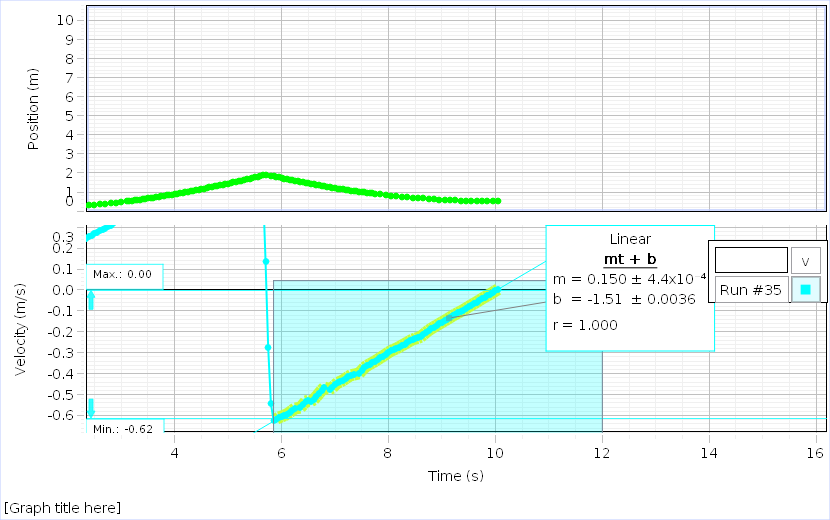
\includegraphics[width=10cm]{Lab2Image3}
\end{center}
Since $m_{\plain{vel}} = 0.150$, we get that the acceleration should be $0.150~\plain{m/s}$, where positive direction means away from the motion sensor.
}\end{document}
